%===================================== CHAP 3 =================================

\chapter{Case Study: The Life Science Building Project}
\section{Introduction of the Life Science Building Project}
The project case will examine the construction of the new life science building of the University of Oslo. When finished, the building will reach a cost of approximately 6,8 million Norwegian Kroner (NOK), and cover 66,700 square meters, with this, becoming the most extensive, detached university building in Norway. Construction builder is the Norwegian Directorate of Public Construction and Property Management (Statsbygg). The construction started on the 8 of February 2019 and is expected to finish in 2024, while the project management of this report started in 2017.

The manager, Stasbygg, is a significant organization in the Norwegian construction industry. They are on a state mission, which means that they are to realize the politics decided by the government, achieved in architecture, cultural legacy, spatial planning, and environment. 

Each year, Statsbygg constructs about 100 construction projects. Some are more complex than others. The life science Building is one of the more complex. In addition to the construction of new buildings and projects, Statsbygg managing about 600 properties of these 90 outside of Norway. Examples of properties managed by Statsbygg are embassies, royal properties, colleges, and cultural buildings. 

In regards to complexity, the new life science building has to meet several complex requirements: (1) the environmental: The property is to achieve Excellent in the BREEAM NOR classification of sustainable properties; (2) usability: a group of the final users has given their feedback on what they expect from the final building; and (3) technical requirements: The building is to house several faculties, some requires highly technical labs.

\subsection{Project Vision and Strategies}
The construcionn of the new Life Science Building is, in many ways, a prestige project. Defined in the vision:
\begin{quotation}
    \textit{"An even better project"}
\end{quotation}
The project is following in the line of previous two large projects running Lean Construction, with Statsbygg as manager. Starting with the Domus Medica construction concluded in 2013. This project was the first Norwegian group applying Lean. This construction was followed by the raising of the new Bergen Academy of Art and Design (BAAD). During these projects, Lean Construction was a significant part of the project management. The first project suffered substantial scope creep, which made the managers take action, applying Lean Design and Systematic Completion \textit{Systematisk Ferdigstillelse} on the BAAD-project. The moves made gave results, and when finished in 2017, the project was by many considered one the most successful (complex) building-constructions completed in Norway.

Based on the the BAAD-project a the \textit{Lean methodology in design and construction}-book \cite{lean_i_praksis} descibing the experience from the project, was made. With the previous history and recomendations from the book, Stasbygg, as a manager, defined five superior strategies in the upcoming LSB-project: 
\begin{enumerate}
    \item The Contract strategy
    \item The Lean strategy
    \item Stretegy of Systematic completion
    \item Digitalization strategy
    \item Logistics strategy
\end{enumerate}
These strategies affect how the project should run and emphasize the focus of the project managers, hopefully leading to a sustainable and productive project. Following are a brief introduction to the different strategies as a context for the case. An holistic view of the strategies in the project are illustrated in figure \ref{fig:strategy}. 

\begin{figure}
    \centering
    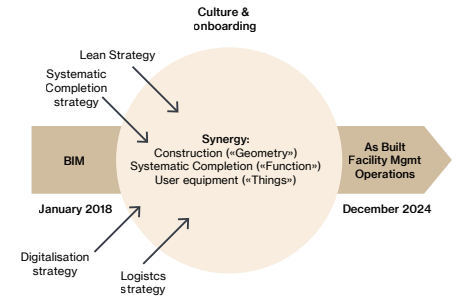
\includegraphics[width=0.8\textwidth]{fig/LVB_strategy.png}
    \caption{A hollistic view of Strategies in the Life Science Building-project.}
    \label{fig:strategy}
\end{figure}

\subsubsection*{The Contract Strategy}
The project has made use of a customized version of the Total Contract, named by Statsbygg as Total Contract with Prior Interaction \textit{(Totalentreprise med forutgående Samspill)}. Instead of signing single contracts with each subcontractor, the managers have assembled eight arrangements, each covering different divisions of the project. Hereunder a more Lead Contract type is applied. Figure \ref{fig:project_contracts}displays the eight contract divisions. Responsible for each of the contracts, from management, is either the project manager from construction or technical. Prior Interaction applies to the design phase, where entrepreneurs are involved prior to the job they are to perform. 

The motivation for this model is, first, shielding the contractors from some of the risk running this project. The project is, as mentioned, very intricate in construction, as well as in management. Moreover, getting contractors willing to apply on this project, the managers will take much of the risk. Regarding cooperation the projects adds Lead Contracts. The intention of this is cooperation; besides, sharing a contract has the plan of shared responsibility and incentives for collaboration between subcontractors. Even though there is a lead contractor per division, the hope is that the group of subcontractors should feel shared responsibility. Why not have a shared responsibility,and no leading contractor, one may ask? The answer is partly laws and politics, but moreover for simplicity in regards to management; a single point of contact. As well, motivation for adding the prior interaction creates a foundation for the Lean strategy.

\begin{figure}
    \centering
    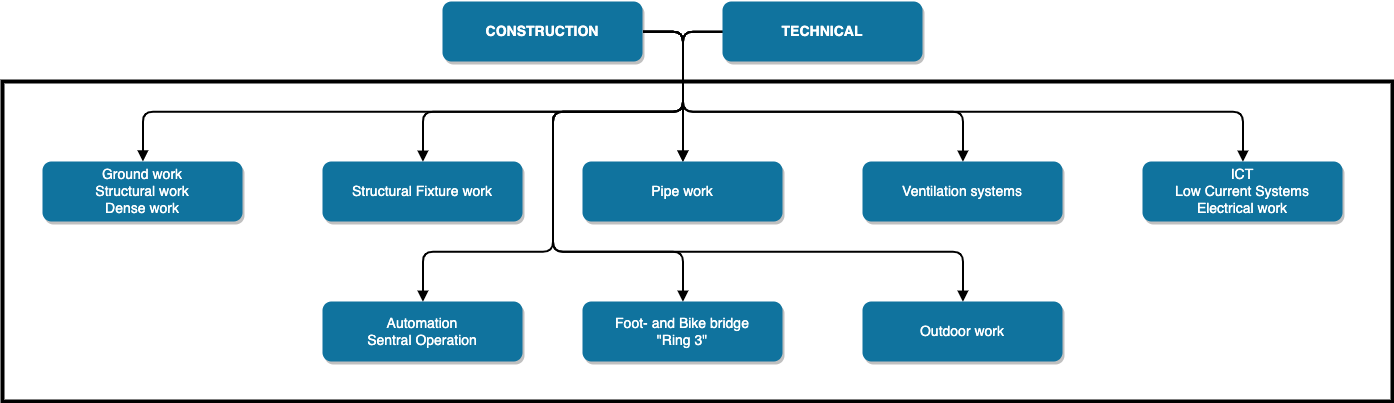
\includegraphics[width=\textwidth]{fig/LVB_contracts.png}
    \caption{Contruction Contracts in the Life Science Building Projects, each managed by either the construction- or technical project manager.}
    \label{fig:project_contracts}
\end{figure}

\subsubsection*{The Lean Strategy}
The Lean Strategy applied in this project is tailor-made from experience from both the Domus Medica- and BAAD-project. Two Lean strategies are applied in the LSB-project: 

\begin{enumerate}
    \item \textbf{Lean Design:} A method conserning design management and design coordination to ensure that the progress and knowledge sharing, in the Design Phase, is as good as possiblble.
    \item \textbf{Lean Construction:} A method conserning the scheduling
    of tasks and the availability of skills and materials to ensure that the work progresses as smoothly as possiblble during the construction.
\end{enumerate}

Different from the traditional design phase described in section \nameref{sec:CI_context}, the LSB-project made use of an iterative method. The \textit{Lean Design}-method has been developed by Statsbygg, after designing the Domus Medica and BAAD projects. In all projects utilizing Lean as their project methodology, this project also iterates over a product. The product, in this context, is the BiM model. The BiM model is the 3-D model of the building. The project makes use of Level of Development (LOD), mentioned in the \ref{sec:lean_construction} section, where each iteration, named sequence, has the intention of getting the BiM model more mature. Also, based on the Contract strategy, the result of this process is not procurement, but the final product ready for implementation - hopefully without bugs. 

A problem with the traditional design phase was evaluating the overwhelming amount of documentation at the end of the phase. Bohem is also mentioning this difficulty when evaluating the waterfall process and problems of use, in his paper mentioned in section \ref{sec:ICT_history}. Furthermore, it is an argument in the Agile manifesto. Having sequences, the Lean Design method, therefore, made it easier having control over all interdisciplinary correlations. In LSB-project, these sequences last up to two weeks. In every sequence, the project leaders are assigned a set of packages. Ending the sequence, the project leaders need to deliver on the packages assigned. This way, the project can identify tasks that are, or can be, risks for the project. Every week in the designing the project starts with a cermony named blackboard-meeting. In this meeting all project leaders, project managers, and responsible goes through the packages and deliveries due to that meeting, or the status if not the end of a sequence. The project chair the meeting, while the rest need to the status of the their area of responsibility. 

The Detail project started with a two-week planning session, which made all trailing package-planning possible. The session resulted in the process map. The process map includes four levels of tasks, illustrated in figure \ref{fig:Milestones-Keypoints-Deliveries-Actions}: (1) the Milestones: A significant planned completion of a part of the project, e.g., steering document approved; (2) Key Points: Key Points is less significant, and with a shorter time frame than milestones, but in the same way an indication of completion; (3) Deliveries: A Key Points consists of several deliveries, e.g., finishing a room or design of a floor; and (4) Actions: Actions is everything needed to be done to complete a Delivery. 

\begin{figure}
    \centering
    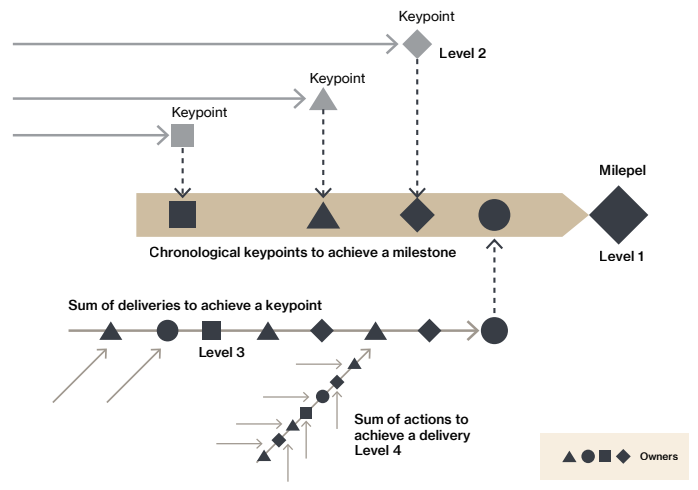
\includegraphics[width=0.8\textwidth]{fig/LSB_task_levels.png}
    \caption{Contruction Contracts in the Life Science Building Projects, each managed by either the construction- or technical project manager.}
    \label{fig:Milestones-Keypoints-Deliveries-Actions}
\end{figure}

Both the Lean Construction, described in section \ref{sec:lean_construction}, and Lean Design, make use of large planing tables. These can look like the old roadmaps used when planning the coding in Waterfall. Depending on how one makes use of the plans, the result of such planes is that they often than not end up wrong. Therefore, as Sutherland points out in his book \cite{sutherland}, the plan is not the final solution, the plan is what is needed, and adapt thereafter. Though, in this case it seems like the time was well spent giving the project leaders valuable insight into the project. Not spendig too much time planning ahed. 

\subsubsection*{The Strategy of Systematic Completion}
As described in section \ref{sec:CI_context}, the construction process ends with the Realization phase. It is after this phase, the project, or building in our case, is tested. If tests run smoothly and the owner approves the construction, the building handover occurs. The mission of testing is to verify that the final product meets the initial requirements and specifications defined. A typical case, when conducting these sorts of tests, is discovering errors. Problems getting wors when there is no control of these errors. If the final construction has too many errors, the owner can decide not to take over the building. Consequently, the project fails to deliver on schedule. Sadly, this happens quite often.

Managing this issue, the LSB-managers has developed a method, checking the systems, functions, and geometry of the construction. The method is named \textit{Systematic Completion} (SC). Throughout the project, SC is conducted, reducing the risk of not deliver the final project. SC follows the LOD-version, which makes for successful completion, with the correct level of quality, at the right time.

\subsubsection*{The Digitalization Strategy}
The Digitalization strategy is, both important in itself, but also supportive in regards to the other strategies. The project using a digital 3-D visualization of the building as the product, driving the Lean Design method. BiM is, in many ways, the core of the project, supported by a dRofus, which is the room database. Prominent in the strategy is connecting all software used in the project and making all entrepreneurs use the same. Hopefully, one can trace the socket implemented in a room, by an electrician, through the drawings given, back to the BiM-model, and the dRofus database, where it was first planned. The resulting system can later be used by janitors, running the building, to identify errors in the system.  Figure \ref{fig:LSB_systems} visualize the connected systems in the project.

\begin{figure}
    \centering
    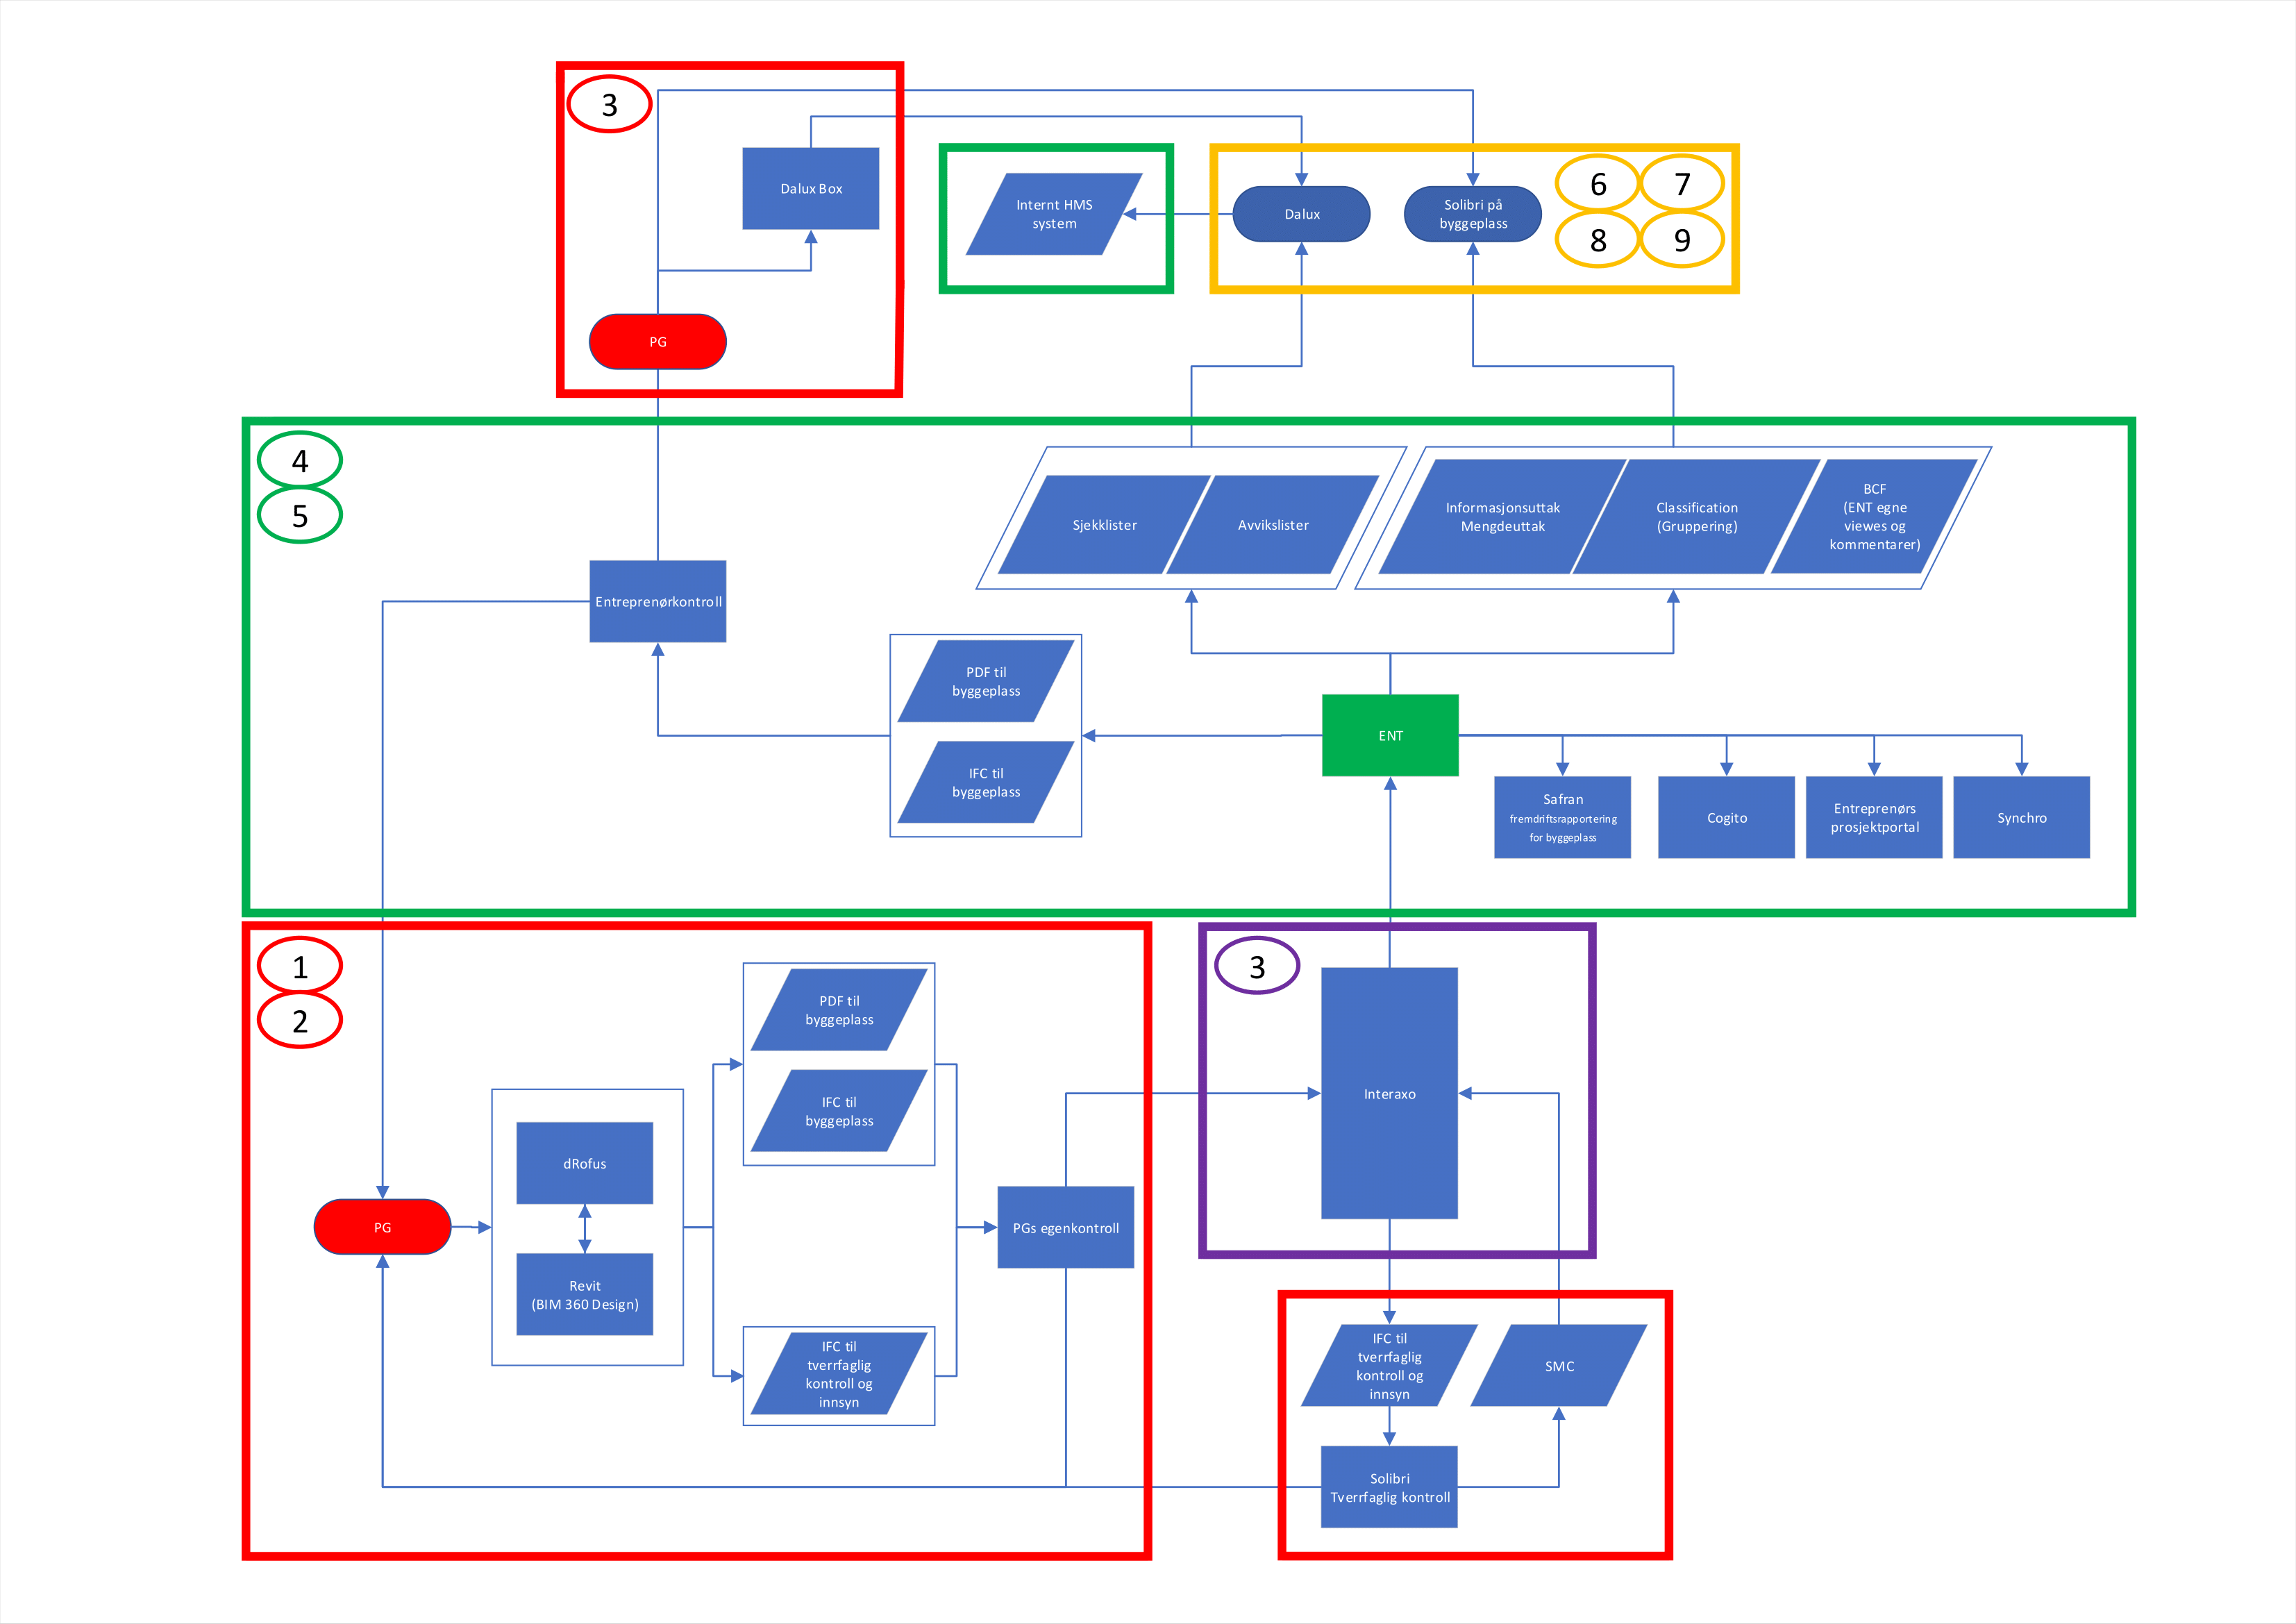
\includegraphics[width=\textwidth]{fig/LVB_system-arkitektur.png}
    \caption{Overview over the system architecture used in the Life Science building project. Outlines representes the actors using the systems, by color: (red) Project group, (green) Entrepreneurs, (yellow) HSE, and (blue) cloud service sharing documents}
    \label{fig:LSB_systems}
\end{figure}

A significant part of the digitalization, and unique for the LSB-project, is the deployment of the Cogito Project-system. Cogito is a tool used to visualize the planning done in the design phase, supporting the Lean Design method. The tool are beeing used tracking actions, deliveries, and Key points and milestones, who is responsible. Furthermore, calculate Planned Percent Completed (PPC), which is an excellent way of identifying delays. The project is planning to use Cogito tracking both the design- and the implementation phase of the project.

The project utilizes, added to Cogito, several other software supporting Agile project management and cooperation. Under following a list of the most crucial software, concerning Agile and collaboration. 

\begin{itemize}
    \item {\bf BiM:} 3-D modeling tool, used in design, constructing, as well as bases for operation when the building is finished.
    \item {\bf Revit and dRofus:} Databases supporting BiM. Whats defined in dRofus is known as the truth, if there is missmatch between BiM and dRofus.
    \item {\bf Interacso:} Cloud service for documents. Servecing omboarding, breach handelig, and offboarding. 
    \item {\bf Blink:} Communication tool. This way intricate can happen rapid and informally, without booking meetings and writing emails.
    \item {\bf Cogito:} Visualization of on going and planned packages, in both the design phase and construction phase of the project.
\end{itemize}

\subsubsection*{The Logistics Strategy}
Last, the Logistics Strategy. When coordinating a large number of people and paraphernalia, having control is a major challenge. In the LSB-project, there will be up to 800 people and equipment worth over 1 million NOK.  These numbers argue for the logistics strategy. The strategy involves planning for goods arriving the lot, as well as where one should tossing the garbage. Considered in this strategy is also removing packaging before arriving the lot, where the goods should arrive, securing the most effective utilization of construction workers. Should the project construct a cantina, so the workers do not have to walk to the nearest McDonald's or grocery store when having lunch? Furthermore, alining workers, equipment, and goods needed to support the train in the Lean Construction strategy. This strategy could be a significant impact when considering the overall labor productivity of the project. 


\subsection{Project management in the Life Science Building-project}
To manage a project, this significant, the constructing organization makes use of several different management approaches. One can divide the project management into two levels: (1) process management: The support of the process and how the teams are working together, and in what order; and (2) implementation management or method management: The management of design and implementation of the final product. The organization structure used in the project supports the two levels of project management. The first of the two, process management, is using customized phase-based process management, inspired by agile thinking. Second, implementation management utilizing the above strategies. 

The construction project organization structure is, as seen in figure \ref{fig:project_structure}. Starting at the top, in charge of the project, is the project director (PD), supported by the assisting project director (APD). The board, seen on the right, consists of four managers, each responsible for different strategies of the project. On the left HSE and project support, which is responsible for i.a. Communication, economics, progress. Beneath the four divisions in the project, where design is responsible for process and management. Paraphernalia is responsible for equipment in the final building. Construction and Technical are two divisions responsible for the eight contracts. In each of the division a Project Leader (PL) is responsible. The PL in Construction and Technical the PLs are responsible for the projects concerning their contracts.

\begin{figure}
    \centering
    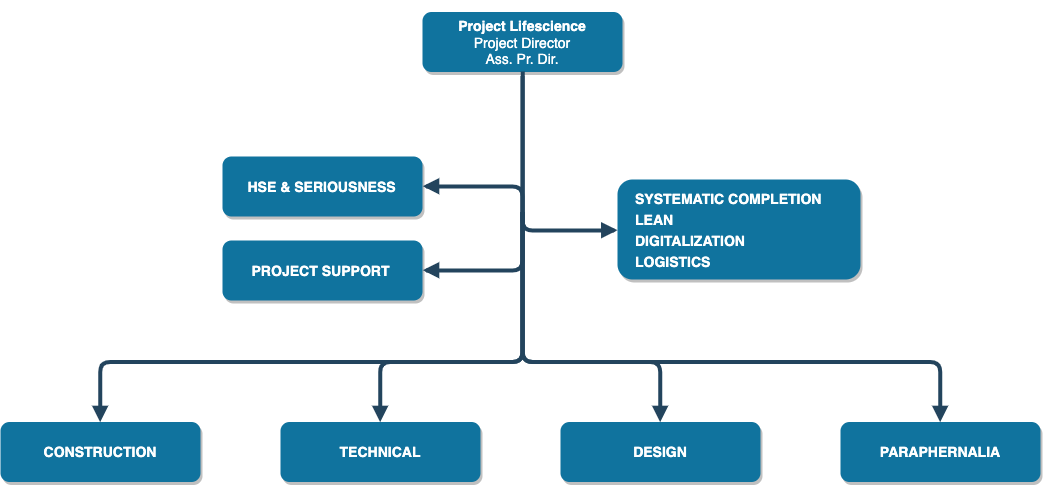
\includegraphics[width=\textwidth]{fig/lvb_diagram.png}
    \caption{Organizational structure in the Life Science Building Project.}
    \label{fig:project_structure}
\end{figure}

\section{Cooperation in the Life Science Building Project}
The LCB-project is, as mentioned, a Norwegian pioneer construction, with a grand vision and intricate strategies, not conducted at this scale before. Running pioneering work is often a conglomeration of trial and error, and the LCB-project is not different. This section will look at the Case and discuss how the project utilizes Lean and supportive software. As well as, how does knowledge sharing work, and what are the problems regarding cooperation in the LCB-project? 

\subsection{The Top-Down Approach}
The LSB-project has, as mentioned two layers of management, and supporting, is the five strategies. Responsible for each part of the project is a PL. Based on the strategies, which the PL are to follow, the project has to be managed using Lean. The Lean methodology in design and construction-book promotes this top-down approach. Arguing that using a bottom-up approach will not give a lasting effect, because the project will, when finished, dissolve. The consequence of using this approach is that the workers often do not feel the same affiliation to the method used. One can argue that a worker should not decide upon which project management method the PLs are using. Looking at it from a software developer's point-of-view, this makes no sense. Sure, making sure that Lean diffusion is essential, but having it work, one needs to involve the workers. 

Concerned by the Lean approach in this project is mostly the PL. One, because of the top-down approach, too, because the ones having any sense of the method is the PLs. They are sheltering the workers who are conduction the modeling, drawing, and designing of the building. Participating in the blackboard-meetings, and using the Cogito tool is the PLs. 

Since this project is such a pioneer project, some of the PLs have never before used Lean. This issue is reflected in what they are saying:  
\begin{quote}
    \textit{"We were told to use it; thus, we are Lean."} - Project Leader, the Life Sciende Building Project
\end{quote}
Proclaiming stupidity is wrong; it is just that they have no experience using Lean. The problem of getting the PLs to know how to utilize the strategies is therefore present. The issue can be seen both in the way they utilize the digital tools, and how they react to the focus on knowledge sharing and transparency. The next section will discuss these issues.

\subsection{Software utilization in the Life Science Building Project}
As we have already seen, the LSB-project has a high degree of technology diffusion. Supported by the Digitalization Strategy, when introducing new technology, it is therefore widespread. When considering the technology infusion, on the other hand, one can not say the result is just as good. Sure, there are some examples where infusion is at a hi degree, BiM, for example. The designers and modelers use BiM, and when the model is complete, the construction workers and installers use the model on the building lot. Cogito, on the other hand, is not that well infused. After all, the software is one of the prestige products of the LSB-project, which makes it odd not utilize it more. Partly this has to do with the top-down approach, but also protecting the designers and modelers from the responsibility. If workers are failing to deliver an action or delivery, it is the PL who will take the blame. Another factor is the fear of knowledge sharing in the CI is very present. This fear comes from the standard way of always protecting the firms' contract. A norm for the contractors, in complex constructions, has been hiring separate personnel responsible for the deviation. 

Essential for the managers in the Lean strategy is the communication between every participant in the project. Blink, the communication platform, was first introduced in the fall of 2019. Almost two years after the detailed design started. Sure, as a project manager pointed out, it is not the tools who make the project Lean. As much as they emphasize cooperation and communication, contra silos, a simple communication tool should have been deployed from the beginning.

When considering technology infusion and defusion in the LSB-project, it seems like the managers have decided on how well defusion and infusion shall be. The problem is for them to make the users see the potential and usefulness of the tools given. For some users, a new digital tool or software is no more than a password and username, that needs to be remembered. This problem is especially present regarding the late deployment of Blink. 

When running a considerable project like the LSB-project, keeping track is key. Cogito supports an overview of which packages currently in production, as well as calculates the PPC. Not available are typical KPIs: how well are the production, what is the status in the current sequence, and what is the LP of the project? One could probably utilize tools such as BiM and Cogito, to produce stats, using these as bases for the proposed KPIs by Skappel. Also, the NORDIC 10-10 tool could be beneficial, analyzing the project performance. 

TODO: 
\begin{itemize}
    \item More on CSCW, and how the LSB-project utilize the software added
\end{itemize}


\subsection{Knowledge utilization in the Life Science Building Project}
As mentioned, vital in the project is communication. A result of communication is knowledge sharing. A whole lot of the software used in the project promotes knowledge sharing. A problem when depending on software to be used as bounding objects is the tacit knowledge needed using the software. This added to the fact that most users feel that new software is a burden, makes for difficult utilization of the digital tools.   

Handle these challenges the digitalization managers have made use of seminars teaching the staff on how to use a particular software. This introduction was enough until new workers had to be on-boarded later in the project. Facing these issues, the managers arranged drop-in-training, where users struggling could come by and ask questions. Sadly these meetings did not went as planed, resulting in zero participants. It was not before a mail invite, showing others struggling with the same issue, that the workers felt the courage to meet up. 

These incidents are prime examples of issues in the CI: (1) people are afraid of showing their weaknesses: their skills have never been questioned, and they are not used to ask for help; and (2) workers are not used to transparency: showing off what has been done during a sequence is therefore uncomfortable for most workers. 

An essential principle of the Agile Manifesto is the face-to-face conversation. In the LSB-project, many conversations happen face-to-face. The architects make use of stand-up meetings. Furthermore, the Lean Design method makes use of the Blackboard-meeting, where PLs, Principals, and managers meet discussing the past sequence. It is in these meetings the second issue, transparency, is very present. When the PLs was asked why some of the packages have not been finished, one could feel the discomfort. Some also try to change the deadline for the deliveries for them to not seem late. Added is the important "Big room", where every diciplines is gethered in one room, promoting interaction and cooperation. 

\subsection{Other Aspects Concerning Cooperation}
In the research, the project asked managers why they utilize Lean in the LSB-project – unexpected answers where given. The common answer was the success of the BAAD-project. Furthermore, when asked why the thought of Lean first appeared, the answer was the ideas of Lean correlated with the experience from prior Construction projects. The will to change, though, originated in this thought: 
\begin{quote}
    \textit{"Why does always building sites appear as a shit holes?"} - Project Leader, the LSB-project
\end{quote}
Moreover, the motivation for Lean Design, on the other hand, originated in the scope creep experienced in the Domus Medica-project, where the Design Phase resulted in errors, and extensive change of design had to be conducted during the realization phase. Even though not articulated, the last reason is similar to the ones discussed in the literature review concerning symptoms for applying agile. Also, in the Lean methodology in design and construction-book, complex construction, leading to extensive, and often bewildering, documentation, adds to the argument of using Lean in constrcutions.  


\begin{itemize}
    \item People management vs process/method management
\end{itemize}


\cleardoublepage